\documentclass[]{memoir}

%\usepackage[a5paper]{geometry}

\usepackage{amssymb}
\usepackage{amsmath}
\usepackage{amsthm}

\usepackage[utf8]{inputenc}
\usepackage[T1]{fontenc}
\usepackage[ngerman]{babel}

%\usepackage{cmbright}
\usepackage[defaultsans]{droidsans}
\renewcommand*\familydefault{\sfdefault}

\usepackage{pifont} % \ding{61} = Death Symbol, cross

\usepackage[]{fancyvrb}

\usepackage{graphicx}

\newtheorem{theorem}{Theorem}[chapter]
\newtheorem{lemma}[theorem]{Lemma}

\theoremstyle{definition}
\newtheorem{definition}[theorem]{Definition}
\newtheorem{example}[theorem]{Example}
\newtheorem{xca}[theorem]{Exercise}

\theoremstyle{remark}
\newtheorem{remark}[theorem]{Remark}



\usepackage{listings}
\usepackage{color}

\definecolor{javared}{rgb}{0.6,0,0} % for strings
\definecolor{javagreen}{rgb}{0.25,0.5,0.35} % comments
\definecolor{javapurple}{rgb}{0.5,0,0.35} % keywords
\definecolor{javadocblue}{rgb}{0.25,0.35,0.75} % javadoc
 
\lstset{language=Java,
basicstyle=\ttfamily \footnotesize,
keywordstyle=\color{javapurple}\bfseries,
stringstyle=\color{javared},
commentstyle=\color{javagreen},
morecomment=[s][\color{javadocblue}]{/**}{*/},
numbers=none,
numberstyle=\tiny\color{black},
stepnumber=1,
numbersep=10pt,
tabsize=4,
showspaces=false,
showstringspaces=false}



\makeindex


\numberwithin{figure}{chapter}%for figures
\numberwithin{table}{chapter}%for tables
\numberwithin{section}{chapter}
\numberwithin{equation}{chapter}
\numberwithin{subsection}{section}

\setsecnumdepth{subsection}

\begin{document}

\frontmatter

% --------------- TITLE PAGE
\thispagestyle{empty}
\begin{flushright}
{\Large Stephan Kesper}
\vskip 3cm
{\fontsize{48}{52} \selectfont Java}
\vskip 1cm
{\Large \textsl{Einführung in Java und JavaFX}}
\vskip 5cm
\today
\vfill
%\includegraphics{../../../License/by-nc-sa.png}
\end{flushright}
% --------------- TITLE PAGE
\newpage


%    Dedication.  If the dedication is longer than a few lines,
%    remove the centering instructions and the line break.
\cleardoublepage
\thispagestyle{empty}
\vspace*{13.5pc}
\begin{center}
  for Alexa
\end{center}
\cleardoublepage

%    Change page number to 7 if a dedication is present.
\setcounter{page}{1}

\tableofcontents
\newpage

\listoffigures
\newpage

\listoftables
\newpage



%    Include unnumbered chapters (preface, acknowledgments, etc.) here.
\include{}

\mainmatter
\pagestyle{plain}

\chapterstyle{veelo}

%    Include main chapters here.

\chapter{Einleitung}

"`Programmieren lernt man am besten an einem Projekt"'. Diese Aussage habe ich oft gehört und mittlerweile glaube ich selbst daran. Denn mit der Syntax einer Sprache kann man (fast) nichts anfangen, solange man nicht weiß, \textbf{wie} man etwas programmieren soll. Man könnte es damit vergleichen, dass man vielleicht schnell lernen kann, welche Funktion die Pedale in einem Auto haben und in welche Richtung man das Lenkrad drehen muss, um das Auto in die entsprechende Richtung zu bewegen. Aber ob man deshalb schon gut Autofahren kann, geschweige denn in eine enge Parklücke kommt, bleibt zweifelhaft.  

Programmieren zu lernen ist ein iterativer Prozess. Man kann am Anfang vielleicht nur ein "`Hallo"' in der Kommando-Shell ausgeben und ist vielleicht darüber schon glücklich oder betrübt in dem Sinne, dass dies eine ziemlich komplizierte Möglichkeit ist, "`Hallo"' zu schreiben. Doch damit fängt alles an. Wenn man das kann, kann man vielleicht auch sehr bald dahin kommen, Berechnungen auszuführen. Kann man dies, versucht man sich an einer Benutzerschnittstelle und beherrscht man diese, probiert man aufwändigere Probleme mit einem Programm zu lösen, und so weiter. Der Kreativität sind keine Grenzen gesetzt und je mehr man programmiert, desto leichter fällt einem das Verständnis komplexerer Fachliteratur über das Programmieren. In diesem Sinne ist auch dieses Buch zu verstehen. Es ist vermutlich nur das erste in einer langen Reihe von Büchern, die Sie lesen werden, um schließlich in die Höhen der Programmierung aufzusteigen -- sofern Sie dahin überhaupt möchten. Unabhängig davon, was Sie von diesem Buch erwarten, hoffe ich, dass Sie soviel Spaß beim Lesen haben, wie ich beim Schreiben hatte. 

\section{Worum geht es?}

In diesem Buch werden Sie einen Einblick in die Programmierung mit Java, sowie einen ersten Blick auf das neue GUI\footnote{GUI = Graphical User Interface}\index{GUI} Framework von Java werfen: JavaFX. Und da ich im vorherigen Abschnitt bereits sagte, dass man am einfachsten Programmieren lernt, wenn man eine Aufgabe zu realisieren versucht, werden wir dies an einem Beispiel tun. 

Falls Sie die Begründung für die Wahl des Projektes, an dem Sie Programmieren lernen sollen, nicht interessiert, können Sie den Rest dieses Kapitels überspringen. Der Inhalt ist zum Verständnis der folgenden Kapitel nicht notwendig. 

In den 80er Jahren tauchten Bücher mit wilden, bunten Mustern auf. Im Zuge dessen wurde immer wieder von einem Paradigmenwechsel in der Wissenschaft geredet. Die Chaos-Theorie\index{Chaos-Theorie} war geboren und mit dem Namen Mandelbrot\footnote{\textbf{Benoît B. Mandelbrot}, *20. November 1924 in Warschau; \ding{61}14. Oktober 2010 in Cambridge, Massachusetts}\index{Mandelbrot, Benoît B.} untrennbar verbunden. Gleichzeitig tauchte eine knubbelige Figur in Abbildungen auf und wurde als Mandelbrot-Menge\index{Mandelbrot-Menge} oder Apfelmännchen\index{Apfelmännchen} bezeichnet. Diese Menge steht in einem direkten Zusammenhang mit den sogenannten Julia Mengen\footnote{\textbf{Gaston Maurice Julia}, *3. Februar 1893 in Sidi bel Abbès, Algerien; \ding{61}19. März 1978 in Paris}\index{Julia Menge}. Der historische Hintergrund soll uns nicht weiter interessieren, was uns dabei interessiert ist, dass in den 80er Jahren immer wieder Computer Programme auftauchten, mit denen man diese Mandelbrot-Menge berechnen konnte. 

Das wirklich erstaunliche an dieser Menge ist nicht ihre Form, die für sich genommen schon komplex und erstaunlich genug wäre. Die Entscheidung, ob ein bestimmter Punkt innerhalb oder außerhalb der Mandelbrot-Menge liegt, kann nicht durch eine einfache Berechnung getroffen werden. Man muss einen Punkt als Parameter einer immer wieder auf sich selbst angewendeten Funktion betrachten. Sollten die Zwischenergebnisse dieser "`Selbstanwendung"' irgendwann so groß werden, dass sie divergieren, also über alle Grenzen wachsen, so gehört der Punkt nicht zur Menge. Man kann also die Elemente der Menge nur durch Ausschluss berechnen, indem man alle Punkte einfärbt, die nicht zur Menge gehören. Übrig bleibt ein Schwarzer Fleck, für den man eigentlich nur sagen kann, dass seine Punkte noch nicht divergiert sind. Färbt man nun die Punkte, die nicht zur Menge gehören in der Art ein, dass der Moment, ab dem sie divergent wurden, die Farbe bestimmt, so erhält man fantastische Bilder. Das, was uns interessiert, sind also die Randbereiche der Mandelbrot-Menge. 

\section{Ein klein wenig Mathematik}

Da wir uns mit der Mandelbrot-Menge beschäftigen, kommen wir um ein paar Definitionen nicht herum. 

\begin{definition}
Wir bezeichnen mit dem Buchstaben $i$ die Wurzel aus $-1$. \index{i}
\begin{equation}
i = \sqrt{-1}
\end{equation}
\end{definition}
Als Motivation betrachten wir die Gleichung
\begin{equation}
x^2 +1=0
\end{equation}
deren Lösung $\pm i$ ist. Diese Erkenntnis war die Inertialzündung zur Entdeckung (oder Definition -- wie man das auch sehen mag) der Komplexen Zahlen.\index{Komplexe Zahl} Man betrachtete weitere Gleichungen, die unter "`normalen"' Bedingungen nicht lösbar waren, jedoch mit Einführung von $i$ sehr wohl.

\begin{definition}
Die Komplexen Zahlen sind zweidimensionale Zahlen
\begin{equation}\label{eq:komplex}
a+i\cdot b
\end{equation}
mit $a,b\in \mathbb{R}$. Man nennt $a$ den Realteil, sowie $b$ den Imaginärteil. Den Multiplikationspunkt lässt man für gewöhnlich weg.  Mit $p=a+i\cdot b$ und $q=c+i\cdot d$ ergeben sich die Rechenregeln wie folgt:
\end{definition}

\begin{equation}\label{eq:cmlxadd}
p+q = (a+c)+i(b+d)\quad \text{Addition}
\end{equation}

\begin{equation}\label{eq:cmlxsub}
p-q = (a-c)+i(b-d) \quad \text{Subtraktion}
\end{equation}

\begin{equation}\label{eq:cmlxmul}
p\cdot q = (ac-bd)+i(ad+bc) \quad \text{Multiplikation}
\end{equation}

\begin{equation}\label{eq:cmlxdiv}
\frac{p}{q} = \frac{ac+bd}{c^2+d^2} + i\frac{bc-ad}{c^2+d^2}\quad \text{Division}
\end{equation}

\noindent Nebenbei bemerkt, werden wir die Division nicht brauchen, sie ist nur der Vollständigkeit halber aufgeführt. Als letztes brauchen wir noch den Betrag einer komplexen Zahl:
\begin{definition}
Der Betrag einer komplexen Zahl ist eine Abbildung 
\begin{equation}
\vert . \vert : \mathbb{C} \longrightarrow \mathbb{R}^+
\end{equation}
von den komplexen Zahlen in die positiven reellen Zahlen. Der Betrag einer komplexen Zahl stimmt für komplexe Zahlen ohne Imaginärteil mit dem Absolutbetrag einer reellen Zahl überein.
\begin{equation}
\vert z \vert = \sqrt{a^2+b^2}
\end{equation}
\end{definition}

Ist man nur an dem Real- oder Imaginärteil einer komplexen Zahl interessiert, so gibt es die Funktionen

\begin{eqnarray}
\mathfrak{Re}(z) &=& a \\
\mathfrak{Im}(z) &=& b
\end{eqnarray}
für $z=a+i\cdot b$.

\section{Die Iteration}
\begin{definition}\index{Iteration}
Wir definieren eine Vorgehensweise, die Iteration über die Funktion $f$ genannt wird, wie folgt: Es sei $z_0$ eine komplexe Zahl. Dann gilt
\begin{equation}
z_{k+1} = f(z_k)
\end{equation}
für $k\in \mathbb{N}$.
\end{definition}

Nehmen wir die folgende Funktion:
\begin{equation*}
f_c : \mathbb{C} \longrightarrow \mathbb{C}
\end{equation*}
\begin{equation}
f_c(z) = z^2+c
\end{equation}
für einen festen Parameter $c$ ist $f_c$ eine komplexe Parabel, die um den Wert $c$ verschoben ist. $f_c$ ist des Weiteren ein Indikator dafür, ob der Parameter $c$ zur Mandelbrot-Menge gehört oder nicht. Dies beschreibt folgende Definition:

\begin{definition}
Wenn wir über $f_c$ iterieren und $z_k$ endlich bleibt, für alle $k\in \mathbb{N}$, dann ist $c$ Element der Mandelbrot-Menge.\footnote{Vielleicht überrascht Sie diese Definition. Besonders, wenn Sie mathematische Vorkenntnisse mitbringen. Denn die übliche Definition ist diese: Eine komplexe Zahl gehört zur Mandelbrot-Menge, wenn ihre zugehörige Julia-Menge zusammenhängend ist. Dies ist zwar die korrekte Definition, aber sie ist für uns hier nicht besonders aussagekräftig, vor allem deshalb nicht, weil wir sonst den topologischen Begriff "`zusammenhängend"' noch erklären müssten, was das Thema dieses Buches weit überschreiten würde.}
\end{definition}

Wir können natürlich nicht für jede komplexe Zahl überprüfen, ob sie für alle $k\in \mathbb{N}$ endlich bleibt. Man setzt sich einfach eine maximale Iterationsanzahl $N$, bis zu der geprüft wird, ob die $z_k$ endlich bleiben und akzeptiert $c$ als Element der Menge, falls $z_N$ endlich ist. Es hat sich gezeigt, dass es ausreicht zu prüfen, ob $\vert z_k\vert <2$ bleibt. Ist dem nicht (mehr) so, werden die folgenden Iterationen zwangsläufig divergieren. 

\section{Die Mandelbrot-Mengen-Iteration}

Aus dem vorherigen können wir nun unsere Berechnungsvorschrift ableiten:

\begin{enumerate}
\item Wähle komplexe Zahlen $c$ beliebig und $z_0=c$, sowie eine maximale Iterationsanzahl von $N\in \mathbb{N}$ und den Iterationsindex $k=0$.
\item Setze $z_{k+1} = f_c(z_k) = z_k^2 +c$
\item Ist $\vert z_{k+1} \vert \ge 2$, breche ab, denn $c$ ist kein Element der Mandelbrot-Menge. Bewahre $k$ auf zur Färbung.
\item Setze $k = k+1$
\item Ist $k\ge N$, breche ab, denn $c$ ist vermutlich ein Element der Mandelbrot-Menge. 
\item Gehe zu (2)
\end{enumerate}

Damit haben wir das theoretische Rüstzeug zur Entwicklung unseres Programms.

\begin{xcb}{Aufgaben}
Im Folgenden ist immer $c=c_1+ic_2$
\begin{enumerate}
\item Sei $z_k = a_k+ib_k$. Berechne $z_{k+1}$ und gib den Real- und Imaginärteil separat an. 
\item Berechne $f_c\left( f_c(z)\right)$ für ein beliebiges $z = a+ib$.
\end{enumerate}

\end{xcb}



\chapter{Grundlagen}

In diesem Kapitel beschäftigen wir uns zunächst mit der Installation und Konfiguration unserer Entwicklungsumgebung, in der wir später programmieren. Leider ist dies ein etwas aufwendiger Prozess und Sie müssen ihn jedes Mal durchgehen, wenn Sie einen neuen Rechner bekommen, oder fatalerweise Ihr Betriebssystem neu installierten. Auch Updates führen manchmal dazu, dass man Teile oder auch den gesamten Prozess neu durch gehen muss. Aber dazu später mehr.

\section{JDK und JRE}

Die Programmiersprache Java\footnote{Oracle and Java are registered trademarks of Oracle and/or its affiliates. Other names may be trademarks of their respective owners. Dies nur als rechtlicher Hinweis.} wurde 1991 bis 1992 von Patrick Naughton, Mike Sheridan, James Gosling und Bill Joy entwickelt (siehe \cite{wikijava}), damals noch bei Sun Microsystems. 2010 wurde Sun von Oracle gekauft. Nun ist Oracle -- nachdem noch weitere Firmen aufgekauft wurden -- im "`Besitz"' der Java Technologie. \index{Java}\index{Gosling, James}\index{Joy, Bill}\index{Sheridan, Mike}\index{Naughton, Patrick}

Java wird in zwei Versionen angeboten. Zum einen dem Java Runtime Environment (JRE). Dieses dient nur zum Ausführen von Java Programmen. Man kann mit dem JRE keine Programme schreiben. Das Programmieren ist mit dem Java Development Kit (JDK) möglich. Zudem enthält das JDK ein vollständiges JRE zur Ausführung der geschriebenen Programme. Das heißt: Ein JDK ist auch ein JRE, aber nicht umgekehrt. \index{JDK}\index{JRE}

Zudem bekommen Sie das JDK und JRE in 32-Bit oder 64-Bit Versionen. Falls Sie nicht einen älteren Prozessor oder sehr wenig Hauptspeicher besitzen, würde ich immer zu den 64-Bit Versionen tendieren. Ich habe zwar keine Untersuchungen darüber angestellt oder gelesen, aber subjektiv habe ich den Eindruck, dass die 64-Bit Java VM schneller ist. Daher empfehle ich diese.

Über die bekannte Seite 

\begin{Verbatim}[fontsize=\small]
https://www.java.com/de/
\end{Verbatim} 
erhalten Sie nur ein JRE. Damit können Sie nicht programmieren. Sie müssen auf folgende Seite gehen:
\begin{Verbatim}[fontsize=\small]
http://www.oracle.com/technetwork/java/javase/downloads/index.html
\end{Verbatim}
oder einfach auf 
\begin{Verbatim}[fontsize=\small]
http://download.oracle.com
\end{Verbatim}
und klicken sich dann zum JDK durch. Falls Sie schon einmal den Begriff Software Development Kit (SDK) gehört haben, so ist das JDK die Java Version eines solchen. 

Sie werden auf der Oracle Seite die Unterscheidung zwischen Standard Edition (JavaSE) und Enterprise Edition (JavaEE) finden. Man würde vermuten, das diese sich nur in der kommerziellen Ausrichtung unterscheiden. Tatsächlich sind dies aber unterschiedliche Technologien. Wir verwenden hier ausschließlich die Standard Edition, \textbf{nicht} die Enterprise Edition. Achten Sie bitte beim Download auf diese Unterscheidung!

Wenn Sie es heruntergeladen und installiert haben, sollten Sie in der Lage sein den folgenden Befehl in der Shell auszuführen:
\begin{Verbatim}[fontsize=\small]
C:>java -version
java version "1.8.0"
Java(TM) SE Runtime Environment (build 1.8.0-b128)
Java HotSpot(TM) 64-Bit Server VM (build 25.0-b69, mixed mode)
\end{Verbatim}

Sollten Sie obige Meldung nicht bekommen, dann müssen Sie Ihre Umgebungsvariablen anpassen, sodass das java.exe Executable gefunden werden kann.

\section{Virtual Machine}

Eine der zentralen Anforderungen an die Java Sprache war von Anfang an, dass die darin entwickelten Programme auf diversen Plattformen ohne Änderung lauffähig sein sollten. 
\begin{quote}
Write once, run anywhere!
\end{quote}
galt als Devise -- von Sun Microsystems. 

Um dieses Ziel zu erreichen, wurde eine Abstraktionsschicht in die Sprache eingebaut. Wie andere Compiler-Sprachen auch, übersetzt ein Java Compiler die von Menschen erzeugten Programme in einen maschinenlesbaren Code. Sprachen wie C, C++, Fortran, usw. erzeugen am Ende einen Code, der auf der Maschine, auf der der Compiler ausgeführt wurde, sehr gut und schnell läuft. Nicht so Java, der vom Java Compiler erzeugte Maschinen Code (Bytecode genannt) ist nur von einem anderen Programm lesbar. Dieses andere Programm liest den Java Bytecode und übersetzt die Bytecode Befehle direkt in Befehle des ausführenden Computers. Das bedeutet, dass dieses ausführende Programm die technischen Besonderheiten des Computers kennen muss, das Java Programm aber nicht mehr. Hat man nun auf verschiedenen Systemen ein solches Programm, das Java Bytecode lesen und ausführen kann, ist die Anforderung erfüllt, dass Java Programme einmal geschrieben und kompiliert werden müssen, dann aber auf allen Computern lauffähig sind, auf denen ein solches Programm, das Java Bytecode lesen und ausführen kann, installiert ist. 

Das "`Programm, das Java Bytecode lesen und ausführen kann"', wird als Java Virtual Machine\index{Virtual Machine}\index{Java Virtual Machine}\index{JVM} bezeichnet. Sie simuliert auf den verschiedensten Systemen, auf denen sie verfügbar ist, immer die selbe, nicht real existierende, Computerumgebung. Für diese Computerumgebung -- die Virutal Machine -- werden Java Programme entwickelt. 

Aktuell steht die Java Virtual Machine auf den Betriebssystemen Windows, Linux und MacOS zur Verfügung. Sowie von IBM eine spezielle Java Virtual Machine sowohl für Windows als auch AIX. Es gab früher mal eine Virtual Machine von Hewlett Packard im HP-UX Umfeld. Ich kann leider nicht sagen, was daraus geworden ist, da ich mit HP-UX nichts mehr zu tun habe. Es ist aber zu erwähnen, dass die Entwicklung einer Java Virtual Machine (JVM) eine recht aufwändige Sache ist und sich daher nur in sehr speziellen Fällen lohnt. Dies musste auch die Apache Foundation einsehen, die mit dem Apache Harmony Projekt eine offene, kostenlose und frei verfügbare Java Virtual Machine schreiben wollte. Im November 2011 wurde entschieden, das Projekt wieder einzustellen. Was -- unter anderem -- dem Umstand geschuldet war, dass mit OpenJDK nach dem Kauf von Sun durch Oracle eine Open Source Implementierung einer JVM verfügbar war. OpenJDK enthält den Source Code der ehemaligen Sun JVM, aus dem die kommerziellen und/oder patentrechtlich geschützten Teile entfernt und durch offene Implementierungen ersetzt wurden. OpenJDK ist vor allem im Linux Bereich die bevorzugte JVM.

Es ist möglich, direkt Bytecode zu schreiben, den eine Virtual Machine ausführt. Dies machen sich andere Sprachen zu nutze, z.B. Scala, die einen Compiler brauchen, aber kein Runtime Envrionment, da sie dann einfach das der JVM nutzen. 

\section{Compiler}

Der zu Java gehörende Compiler heißt \texttt{javac}\index{javac}. Machen wir mal ein kleines Experiment. Erzeugen Sie ein Verzeichnis und legen dort eine Datei an mit dem Namen \texttt{Test.java}. Öffnen Sie diese Datei in einem Editor und schreiben Sie folgenden Text hinein:

\begin{lstlisting}
public class Test {
  public static void main(String[] args) {
    System.out.println("Hello World!");
  }
}
\end{lstlisting}\label{code:test}\index{Hello World!}

Speichern Sie die Datei und schließen Sie sie. Öffnen Sie nun eine Kommandoshell in dem selben Verzeichnis und rufen Sie den Compiler auf mit 
\begin{Verbatim}
javac Test.java
\end{Verbatim}
Der Compiler wird wortlos die gewünschte Aktion durchführen. In Ihrem Verzeichnis sollte nun zusätzlich eine \texttt{Test.class} Datei erzeugt worden sein. Rufen Sie danach 
\begin{Verbatim}
java Test
\end{Verbatim}
auf, es sollte ein "`Hello World!"' erscheinen. Glückwunsch: Ihr erstes -- so hoffe ich -- Java Programm.

Der Aufruf des "`java"' Programms vor Ihrem "`Test"' Programm ist der Aufruf der JVM. Die JVM ist die java.exe, die dann Ihr Programm im Bytecode ausführt. Sie haben damit ein "`Hello World!"' Programm geschrieben, dass sowohl auf Windows, Linux als auch MacOS lauffähig ist. Ist doch gar nicht so schlecht, oder?

Wir werden es hierbei schon mit Informationen über den Compiler belassen. Wir kommen später noch einmal darauf zurück. 

\section{IDE}

Üblicherweise programmiert und kompiliert man nicht mit einfachen Editoren und einer Shell. Sie können es, gar keine Frage. Aber angenehm ist das nicht. 

Zur Entwicklung bedient man sich meistens besonderer Programme, die das Entwickeln von Software einfacher machen. Sogenannte Integrated Development Environments (IDE). \index{IDE}\index{Integrated Development Environment}

Im Java Umfeld gibt es diverse IDE's, hier sei nur auf die bekanntesten und gleichzeitig kostenlosen hingewiesen. 

\begin{enumerate}
\item Eclipse (\texttt{http://www.eclipse.org})\index{Eclipse}
\item Netbeans (\texttt{http://www.netbeans.org})
\item IDEA IntelliJ Community Edition (\texttt{http://www.jetbrains.com})
\end{enumerate}
Von Jetbrains\index{Jetbrains} gibt es auch eine kommerzielle Version ihrer IDEA IntelliJ Umgebung, die Community Edition ist aber kostenlos.

Wir werden uns hier auf die Netbeans IDE\index{Netbeans} beschränken. Das hat zum einen den Grund, dass alle Funktionalitäten der Netbeans IDE kostenlos sind. Das gilt zwar auch für Eclipse, aber seit dem Upgrade auf die Version 4.0 habe ich persönlich die Freunde an Eclipse verloren. Das verschiedene Gründe, die ich auf Rücksicht und Respekt vor der vielen Arbeit der Eclipse Entwickler, für mich behalte. Sagen wir einfach, ich hätte eine Münze geworfen.

Ich möchte Sie hier an dieser Stelle ermutigen, sich alle Entwicklungsumgebungen einmal zu installieren und genau auszuprobieren. Vielleicht gefällt Ihnen ja eine andere besser und Sie kommen gut damit zurecht. Jede hat ihre Stärken und Schwächen. Ich selbst verwende oft verschiedene IDE's für verschiedene Zwecke.

\subsection{Installation}
Der Installer von Netbeans\footnote{Wir verwenden hier die Netbeans Version 8.0} ist schnell herunter geladen und zum Setup brauchen Sie im allgemeinen keine zusätzlichen Informationen. Die Einstellungen sollten auf den Vorgabe Werten belassen werden. Sofern Sie bereits ein JDK installiert haben, wird Netbeans dies automatisch finden. Sollte es hier Schwierigkeiten geben, oder Sie erst später das JDK installiert haben, müssen Sie folgende Einstellung vornehmen:

Suchen Sie im Netbeans Installationsverzeichnis die netbeans.conf Datei
\begin{Verbatim}
C:\Program Files\NetBeans 8.0\etc\netbeans.conf
\end{Verbatim}
Dort sollten Sie die Angabe
\begin{Verbatim}
netbeans_jdkhome="C:\Program Files\Java\jdk1.8.0"
\end{Verbatim}
finden. Sollte diese Angabe falsch sein, oder nicht zu Ihrem JDK passen, sollten Sie diese Einstellung anpassen.
Ich bin hier davon ausgegangen, dass Sie ein 64-Bit JDK und die 64-Bit Version von Netbeans installiert haben. Diese beiden müssen zueinander passen. Haben Sie das 32-Bit JDK installiert, müssen Sie auch die 32-Bit Version von Netbeans installieren. Sonst bekommen Sie Schwierigkeiten.

Wenn Sie Netbeans zum ersten Mal starten, bekommen Sie die Start Page angezeigt. Sie erscheint im Editor Fenster und kann durch das kleine Kreuz am Namensreiter geschlossen werden. Ist diese geschlossen, haben Sie einen Blick auf die leere IDE. 

\subsection{Projekte}

Alle IDE's arbeiten in sogenannten Projekten.\index{Projekt} Sie können sich ein Projekt als ein Verzeichnis mit darin enthaltenen Dateien vorstellen. Nicht nur Ihre Java Dateien werden darin liegen, sondern auch alle Projekt-spezifischen Einstellungen der IDE. Abbildung \ref{nb:newproj} zeigt den Wizard, mit dem man ein neues Projekt anlegen kann. Klicken Sie auf "`next"', wählen Sie den Haken ab, eine "`Main-Klasse"' zu erzeugen und geben Sie dem Projekt einen Namen, zum Beispiel "`TestApplication"'.

\begin{figure}[h]
\centering
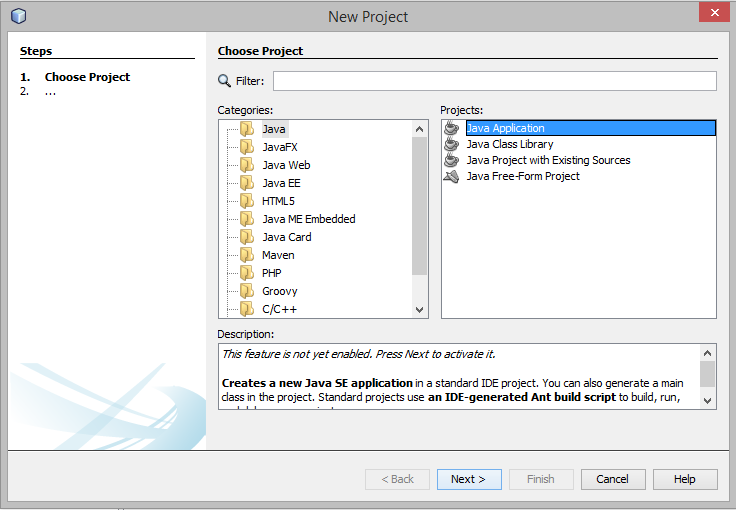
\includegraphics[width=\textwidth]{img/nb001}
\caption{Wizard zur Erzeugung eines neuen Java Projekts}
\label{nb:newproj}
\end{figure}

Wenn Sie das Projekt angelegt haben, sollte Ihr Projekt so wie in Abbildung \ref{nb:emptproj} aussehen.

\begin{figure}[h]
\centering
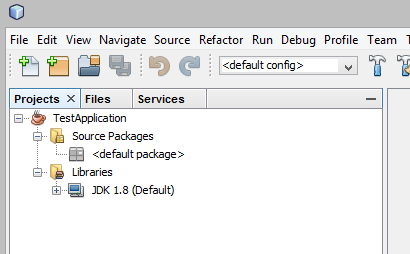
\includegraphics[]{img/nb002}
\caption{Leeres, neues Java Projekt}
\label{nb:emptproj}
\end{figure}

\newpage
Wenn Sie auf den "`Source Package"' Order mit der rechten Maustaste klicken, erscheint das Kontext Menü. Wählen Sie "`New $\rightarrow$ Java Class ..."' und füllen Sie den Wizard so aus, wie in Abbildung \ref{nb:newclass}.

\begin{figure}[h]
\centering
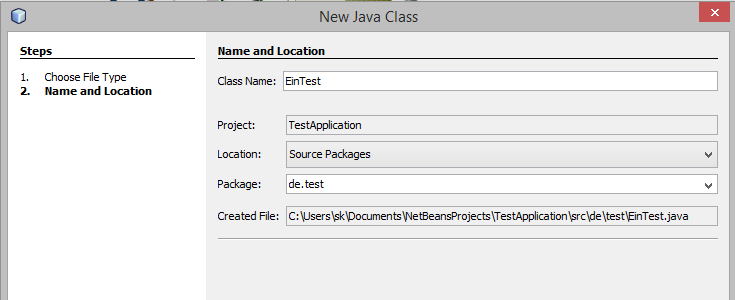
\includegraphics[width=\textwidth]{img/nb003}
\caption{Neue Klasse}
\label{nb:newclass}
\end{figure}

Danach sollte in Ihrem Editor ein Fester auf gehen, mit dem folgendem Inhalt 

\begin{lstlisting}
/*
 * To change this license header, choose License Headers in Project Properties.
 * To change this template file, choose Tools | Templates
 * and open the template in the editor.
 */
package de.test;
/**
 *
 * @author kesper
 */
public class EinTest {
    
}
\end{lstlisting}
Die Zeilen, die mit den *-Zeichen beginnen, sind Kommentare. In Java (und auch anderen Sprachen) sind Kommentare Informationen für den Entwickler, sie werden vom Compiler grundsätzlich ignoriert. Es gibt zwei Arten von Kommentaren, nämlich den einzeiligen und den begrenzten Kommentar. \index{Kommentar}

Einzeilige Kommentare beginnen mit zwei Slash-Zeichen "`//"'. Sie können an jeder beliebigen Stelle im Source Code auftauchen und gelten immer bis zum Ende der Zeile. Das heißt, alles in einer Zeile, das hinter zwei Slash-Zeichen steht, ist ein Kommentar, auch wenn Sie nach dem Kommentar noch Code einfügen wollen, geht das nicht, es wird auch weiterhin als Kommentar betrachtet. 

Der begrenzte Kommentar hat Start- und Stopp-Symbole. Slash Stern(\texttt{/*}) öffnet einen Kommentar und Stern Slash (\texttt{*/}) schließt ihn wieder. Auch wenn es sich bei dem Kommentar nur um ein Wort handelt, können Sie nach einem begrenzten Kommentar -- selbst in der selben Zeile -- weiterschreiben. Sollten Sie einen längeren Kommentar einfügen wollen, lohnt sich der begrenzte Kommentar immer. 

Kommentare werden Ihnen am Anfang unsinnig erscheinen. Wenn Sie aber eine Weile programmieren und ältere Code Stücke analysieren möchten, werden Sie für Kommentare -- sofern sie beschreiben, was Sie sich beim Erzeugen des Codes gedacht hatten -- sehr dankbar sein.

In Java haben bestimmte Kommentare noch eine weitere Funktion: Sie dienen der Dokumentation Ihres Codes. Solche Kommentare, die mit "`/**"' Slash-Doppelstern beginnen, gehören zum sogenannten Javadoc\index{Javadoc} System. Dies ist eine recht elegante Art, wie Sie innerhalb Ihres Source Codes Kommentare schreiben und diese automatisiert zu einer HTML Dokumentation zusammen fügen lassen können. Dies wird später noch genauer erklärt.  

\subsection{Packages}
Als nächstes fällt auf, dass am Anfang des Codes eine Paket Anweisung steht. Packages (dt. Pakete)\index{Package}\index{Paket} sind Ansammlungen von Klassen. Es ist zwar möglich Klassen ohne Package zu erzeugen, das hatten wir mit der Test Klasse in Kapitel \ref{code:test} so gemacht, aber dies stellt eine schlechte Angewohnheit dar. Warum, werden wir im Folgenden sehen. Aus unserem Code Pakete zu schnüren hat zwei grundlegende Motivationen: 

\begin{description}
\item[Füge zusammen, was zusammen gehört]
Wenn sich verschiedene Klassen mit dem selben oder Variationen des selben Themas beschäftigen, ist es sinnvoll diese in ein Paket zusammen zu stellen. Alleine der Ordnung willen. Suchen Sie dann eine Klasse, finden Sie sie dort, wo sie sie vermuten könnten, nämlich dort wo alles liegt, was zu dem Thema gehört. 
\item[Bibliothekten]
Wenn Sie später einmal sogenannte Bibliotheken schreiben, also Code Teile, die Sie nicht in verschiedenen Projekten neu entwickeln, sondern wiederverwenden möchten, ist es sehr viel einfacher Kollisionen zu verhindern, in dem Sie Packages verwenden. Genauso ist es einfacher alle Klassen, die zu einem Package gehören in eine Bibliothek zusammenzuführen, wenn man sie anhand ihres Paketes identifizieren kann. 
\end{description}

Packages sind ein Ordnungsprinzip und gleichzeitig trennen sie sogenannte Namensräume. Sie können zwei oder mehr Klassen mit dem selben Namen haben, wenn diese in verschiedenen Paketen liegen. Nicht das Sie dies tun sollten, aber Sie \textit{könnten}, wenn Sie verschiedene Pakete verwenden.

Ein Paket besteht aus einem einfachen, frei wählbaren Namen. Es dürfen allerdings keine Sonder- oder Leerzeichen enthalten sein, sowie darf keine Zahl am Anfang des Paketnamens stehen. Pakete haben eine Hierarchie, das bedeutet, dass es Pakete in anderen Paketen gibt. Dies wird so dargestellt, dass ein Punkt zwischen Eltern Paket und aktuellem Paket geschrieben wird. In unserem Beispiel haben wir das oberste Paket mit "`de"' bezeichnet, so wie es von Sun einmal empfohlen wurde. Danach kommt unser Paket test, in dem wir unsere Klasse angelegt haben. Die sogenannte Signatur unseres Paketes ist also "`de.test"'. 

Die Standard Bibliothek von Java enthält viele nützliche Klassen. Diese sind alle in ihre eigenen Pakte und Unter-Pakete einsortiert. Sie beginnen mit "`java."' bzw. "`javax."'. Sie können keine eigenen Pakete erzeugen, die mit "`java."' oder "`javax."' beginnen. Dies verhindert der Compiler, weil diese Pakete reserviert sind.

\section{Aufgaben}
\begin{enumerate}
\item Was ist der Unterschied zwischen einem JDK und einem JRE?
\item Was ist eine Virtual Machine?
\item Wofür steht die Abkürzung IDE?
\item Was ist ein Package?
\end{enumerate}



\chapter{Klassen}

In diesem Kapitel geht es in erster Linie darum zu erklären, was Klassen sind und wie sie (programmtechnisch) Verwendung finden. Ihre Herkunft und den theoretischen Hintergrund von Klassen im Abstraktionsmechanismus der objektorientierten Programmierung werden wir in Kapitel \ref{chap:oop} kennen lernen.

\section{Objekte und Instanzen}

\subsection{Was ist eine Instanz?}\label{ref:instance}\index{Instanz}

Ein Begriff, welcher dem der Instanz am nächsten kommt, ist "'temporäres Exemplar"'.\index{Exemplar, temporär} In der Biologie sind Exemplare – wie z.B. Eichhörnchen oder Pusteblumen – einzelne Lebewesen. Sie können über die Klasse der Säugetiere reden, aber wenn Sie einen Löwen vor sich sehen, sollten Sie über dieses spezielle Exemplar nachdenken (als gut gemeinter Rat). Das selbe gilt für die informationstechnischen Exemplare. Und als temporär sind diese Exemplare zu verstehen, weil sie eine strikt begrenzte „Lebensdauer“\index{Lebensdauer} haben. Den Begriff Lebensdauer möchte ich nicht formal definieren. Ich glaube, es ist klar, was damit gemeint ist, solange von biologischen Exemplaren die Rede ist. Informationstechnische Exemplare haben ebenfalls etwas das als Lebensdauer verstanden werden kann, nämlich die Zeitspanne zwischen ihrer Erzeugung, d.h. der Zuweisung eines bestimmten Bereichs des Hauptspeichers eines Computers bis zur Zerstörung, d.h. Freigabe des Hauptspeichers der diesem Exemplar zugewiesen war. Als Hinweis, Instanzen können noch in sogenannten „serialisierten“ Zuständen ihre Lebensdauer in einem persistenten Zustand fristen. Dies wird später noch genauer erklärt. 

Exemplare sind spezielle, existierende Dinge, die klassifiziert werden können. An dieser Stelle sollten Sie sich nicht zu sehr an den Begriff Klasse orientieren, denn der wird später noch erklärt. Zwar sind Objekte Instanzen von Klassen, aber der Instanz Begriff sollte hier weiter gefasst verstanden werden. Denn Klassen können ihrerseits wieder Instanzen von anderen Dingen sein, sogenannten Meta-Klassen. Und wenn Sie Computer-Rollen-Spiele kennen, werden Ihnen „Instanzen“ als spezielle Teile eines Dungeons untergekommen sein, die ihrerseits wiederum Instanzen einer abstrakten Dungeon Beschreibung sind. Das vorletzte Vorkommen von Instanz habe ich in Anführungsstriche geschrieben, da die Hersteller von Computer-Rollen-Spielen vermutlich eine eigene Definition vom Begriff Instanz haben. In der hier hergestellten Interpretation des Begriffs passt die temporäre, für eine Gruppe von Spielern hergestellte Kopie eines Dungeons aber recht gut. Fassen wir hier in einer Auflistung kurz die wesentlichen Eigenschaften einer Instanz zusammen: 

\begin{enumerate}
\item Eine Instanz ist klassifizierbar -- in welcher Weise dies geschieht ist nicht definiert!
\item Sie ist ein „real“ existierendes Exemplar -- sofern der Begriff real auf Objekte im Hauptspeicher eines Computers angewendet werden kann.
\item Ihre Existenz ist zeitlich begrenzt
\end{enumerate}


\subsection{Was ist ein Objekt?}\index{Objekt}

Im Grunde reden Sie bei einem Objekt immer von einer Instanz. Diese Begriffe sollten synonym verwendet werden. Warum ich hier einen eigenen Abschnitt für Objekte einfüge und nicht einfach bei Instanzen die Bemerkung fallen lasse, dass Objekte Instanzen sind, liegt darin begründet, dass die Verwendung des Begriffs Objekt oft sehr schwammig ist. Viele Programmierer werfen mit Floskeln um sich wie z.B. „alles ist ein Objekt“. Aber auch der Begriff „Objektorientierte-Programmierung“ ist schon so ungenau in seiner Verwendung, dass die ursprüngliche Definition kaum noch darin auszumachen ist. 

Konsequent lautet die ISO Definition des Begriffs "`objektorientiert"' (siehe \cite{isooo}):\index{objektorientiert}

\begin{quote}
Bezieht sich auf eine Technik oder Programmiersprache, welche Objekte, Klassen und Vererbung unterstützt.
\end{quote}

Na prima. Dem entgegen stehen objektorientierte Sprachen, die keine Klassen brauchen (Prototypenbasierte Programmierung; JavaScript) sowie der Umstand, dass dem Vererbungsbegriff heute nicht mehr die Bedeutung zu kommt, wie noch am Anfang der Euphorie. 

Abgesehen von dem ganzen Durcheinander, das mit den Begriffen "`objektorientiert"' und "`Objekt"' angestellt wurde, reicht es für uns zu wissen, dass ein Objekt (oder eine Instanz) ein Ding ist, das sich im Hauptspeicher unseres Rechners (genauer gesagt des virtuellen Rechners JVM) befindet und unter einem Namen angesprochen werden kann. Dieser Name ist eine sogenannte Referenz (englisch Pointer), der auf einen Bereich des Hauptspeichers verweist. 

\section{Klassen}\index{Klasse}

Eine Klasse ist zunächst einmal nicht mehr als ein Name mit einer öffnenden und einer schließenden, geschweiften Klammer. Die Minimale Klasse, die man definieren kann ist:
\begin{lstlisting}
class Person {
}
\end{lstlisting}
Des Weiteren können Klassen Variablen Definitionen enthalten -- bei Klassen heißen diese dann "`Member"', sowie Funktionen, die innerhalb der Klasse definiert werden. Beispiel:\index{Member}
\begin{figure}[h]
\begin{lstlisting}
class Person {
  private int age;

  public int getAge() {
    return age;
  }
  
  public void setAge(int value) {
    age = value;
  }
}
\end{lstlisting}
\caption{Eine sehr einfache Klasse}
\label{code:class}
\end{figure}

Ok, hier haben wir schon einige Dinge gleichzeitig gemacht, die ich der Reihenfolge nach erklären möchte.

\subsection{Member}\index{Member}
Gehen wir einen Schritt zurück und überlegen, was mit dem Begriff "`Variable"' gemeint ist. Variablen sind Namen für (noch) nicht bekannte Werte. Genauso, wie wir sie bei der Definition der komplexen Zahlen verwendet haben in der Einleitung in Formel (\ref{eq:komplex}). Dort haben wir die Variablen $a$ und $b$ als reelle Zahlen definiert, deren Wert völlig unbestimmt ist. Wir wissen lediglich welcher "`Art"' oder welchen Typs diese Variablen sind. Dies ist Teil des sogenannten Typ-Konzept von Java. Jeder Variable muss ein sogenannter Typ zugewiesen sein, damit Java mit ihnen umgehen kann. Dies dient zum einen dazu, damit immer ausreichend Speicher für die Werte einer Variable beantragt werden kann, sowie auch zu Ihrer eigenen Sicherheit, dass Sie wissen, was Sie mit einer Variablen tun können. Es ist zum Beispiel unsinnig einen ganzzahligen Wert zu einer Zeichenkette hinzu zu summieren und zu erwarten, dass eine Fließkommazahl dabei heraus kommt, darüber beschwert sich dann der Java Compiler (zu recht) in Abbildung \ref{nb:typeerror}.

\begin{figure}[h]
\centering
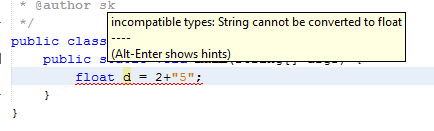
\includegraphics[]{img/nb004}
\caption{Typ Fehler im Netbeans Editor}
\label{nb:typeerror}
\end{figure}

Netbeans beschwert sich, dass die Zeichenkette (in englisch String) nicht zu einem "`float"' konvertiert werden kann. Diese Fehlermeldung sagt uns zwei Dinge. Zum einen, dass man nicht einfach so einen String zu einem Zahlenwert machen kann, auch wenn wir der Anschauung nach glauben, die 5 in den Anführungsstrichen sei ja nichts anderes als eine Zahl. Und zum zweiten, dass die ganze Zahl 2 sehr wohl automatisch zu einer Fließkommazahl konvertiert werden kann. Auf dieses Thema werden wir noch in Kapitel \ref{ref:conversion} zurück kommen.

\subsubsection{Primitive Datentypen}\index{Primitive}\index{primitive Datentypen}
In Java gibt es folgende primitive (d.h. nicht als Klasse dargestellte) Datentypen:

\begin{description}
\item[boolean] 1 Bit, true/false
\item[byte] 8 Bit
\item[char] x Bit, kann ein UTF-8 Charakter sein und somit von nicht vorherbestimmter Länge.
\item[short] 16 Bit, kurzer Ganzzahlwert
\item[int] 32 Bit langer Ganzzahlwert
\item[long] 64 Bit langer Ganzzahlwert
\item[float] 32 Bit langer Fließkommawert im IEEE 754 Standard
\item[double] 64 Bit langer Fließkommawert im IEEE 754 Standard
\end{description}

Ganzzahlwerte sind suggestiver weise Zahlen, die keine Nachkommastellen besitzen. Fließkommawerte sollten vielleicht etwas näher erklärt werden, denn sie sind nicht einfach Zahlen mit Nachkommastellen. Der Wert einer Fließkommazahl ist auf den Bereich zwischen +10 und -10 "`normiert"'. Das bedeutet, jede beliebige Dezimalzahl wird so dargestellt, dass man sie solange mit 10 multipliziert oder durch 10 dividiert, bis sich eine Zahl zwischen +10 und -10 ergibt. Die Anzahl der Multiplikationen oder Divisionen mit 10 merkt man sich in einer zweiten Zahl. Die normierte Zahl zwischen -10 und +10 wird "`Mantisse"' genannt, während die Anzahl der Multiplikationen oder Divisionen "`Exponent"' genannt wird. Diese Darstellung wird auch oft als Ingenieursdarstellung bezeichnet. Beispiel:\index{Fließkommawert}\index{Ganzzahlwert}
\begin{equation*}
1.03888E-12 = 1.03888\cdot 10^{-12} = 0.00000000000103888
\end{equation*}

Der IEEE\footnote{\textbf{Institue of Electrical and Electronics Engineers}\index{IEEE}, meistens als "`I tripple E"' bezeichnet.} 754 Standard bestimmt für 32 Bit Werte eine 23 Bit lange Mantisse sowie einen 7 Bit langen Exponenten und für 64 Bit Werte eine 52 Bit lange Mantisse sowie einen 10 Bit langen Exponenten. Jeweils ein Vorzeichen Bit für Mantisse und Exponenten müssen hinzugerechnet werden.

Für alle oben dargestellten primitiven Datentypen gibt es sogenannte Wrapper Klassen, wie in Tabelle \ref{tab:wrapper} aufgeführt.

\begin{table}[h]
\centering
\begin{tabular}{r|l}
\hline
Primitiv & Wrapper \\
\hline
boolean & Boolean \\
byte & Byte \\
char & Character \\
float & Float \\
int & Integer \\
long & Long \\
short & Short \\
double & Double \\
\hline
\end{tabular}\\[3mm]
\caption{Wrapper Klassen der primitiven Datentypen} \label{tab:wrapper}
\end{table}

Wie Sie sehen, brauchen Sie für die Nutzung der Wrapper (abgesehen von char und int) lediglich den ersten Buchstaben zu ändern. Die Typen char und int wurden (vermutlich) deswegen nicht character und integer genannt, weil in der Programmiersprache C diese Datentypen auch char und int heißen. Und da die Syntax von Java sich an C und C++ orientiert, blieb es wohl dabei.

\subsection{Funktion}\index{Funktion}
Klassen stellen eine Kombination von Daten und Funktionalität dar. Wobei es sinnvoll ist, die Funktionalität nicht von den Daten zu trennen, sondern sie im Gegenteil daraufhin abzustimmen. Klingt etwas kompliziert, ist aber ein relativ einfacher Vorgang. Nämlich anstatt dass auf die Variablen einer Klasse jeder Zugriff hat, versteckt man sie. Dies geschieht mit dem Zusatz "`private"' an der Variablen. Auf eine als privat deklarierte Variable kann von keinem anderen Code zugegriffen werden, als von der Klasse selbst, zu der die Variable gehört. Mehr dazu im Kapitel \ref{chap:encapsule}. Sie ist somit ein exklusives Mitglied (Member) einer Klasse. Und sie stellt in einem gewissen Sinn den Status dar, welcher nur über die Zugriffs-Funktionen verändert werden kann. In unserem Beispiel die \texttt{getAge()} und \texttt{setAge()} Funktionen der Klasse in Abbildung \ref{code:class}. 

Auf diese Zugriffsfunktionen (oder Methoden) beschränkt sich natürlich nicht das Spektrum der Funktionen. In diesen Funktionen wird die eigentliche Arbeit erledigt, für die man Programme im allgemeinen benutzt. Daher lohnt es sich, diese etwas genauer anzusehen:

Funktionen bestehen aus vier Teilen: Einem Namen, unter dem sie angesprochen werden, einer Liste von sogenannten Parametern, einem Rückgabewert und einer Implementierung. Eine Funktion wird immer so aussehen:
\begin{lstlisting}
<Typ> name(Typ parameter1, Typ parameter2, Typ parameter3) {
}
\end{lstlisting}




\section{Instanziierung}\index{Instanziierung}

Wir hatten in Abschnitt \ref{ref:instance} gelernt, was eine Instanz ist. Und dabei definiert, dass Instanzen in einem gewissen Sinne klassifizierbar sind. Dies wollen wir hier nun konkretisieren. Im vorherigen Abschnitt haben wir erklärt, was eine Klasse ist. Doch sind Klassen keine temporäre Exemplare, wie wir dies für Instanzen festgestellt hatten. Klassen sind eher Schablonen, anhand derer ihre temporären Exemplare (oder halt eben Instanzen) hergestellt werden können. Für die Instanzen wird dann vom Runtime Environment Speicher besorgt und zugewiesen. Und zwar genau so viel, wie die Klasse definiert hatte. In diesem Speicher legt die Instanz die Werte ihrer Variablen ab. In unserem Beispiel wäre das nur ein Integer für das Alter einer Person. Die Erzeugung einer Instanz anhand einer Klassen-Schablone wird Instanziierung genannt.\index{Instanziierung}

Wie sagt man nun der Virtual Machine, dass man Speicher für eine bestimmte Instanz haben möchte? Dies geschieht mit dem sogenannten "`new"'-Operator.\index{new}\index{new Operator} Der new-Operator fragt nach Speicher und weist diesen, in der zur Klasse passenden Größe, einer Variablen zu, z.B.:
\begin{lstlisting}
Person p = new Person();
\end{lstlisting}
Unter dem Namen "`p"' können wir ab diesem Moment auf diese spezielle Instanz zugreifen.

Klassen sind also die Beschreibungen der inneren Struktur von Instanzen. Man sagt demnach auch ein bestimmtes Objekt sei die Instanz einer bestimmten Klasse. 

Es ist wichtig zu verstehen, dass die verschiedenen Instanzen einer Klasse sich den Code der Klassen-Funktionen teilen. Also nicht jedes Objekt hat seine eigenen \texttt{getAge()} und \texttt{setAge()} Funktionen. Alle Objekte teilen sich diese "`Implementierung"'. Ändert man die Implementierung, ändert sich das Verhalten aller Objekt dieser Klasse. Das gilt wiederum nicht für die Variablen. Jedes Objekt hat seine eigene Kopie der von der Klasse definierten Variablen. 

\noindent Erweiterten wir die Person-Klasse aus unserem Beispiel:

\begin{lstlisting}
class Person {
    private String firstName;
    private String lastName;
    private int age;

    public String getFirstName() {
        return firstName;
    }

    public void setFirstName(String firstName) {
        this.firstName = firstName;
    }

    public String getLastName() {
        return lastName;
    }

    public void setLastName(String lastName) {
        this.lastName = lastName;
    }

    public int getAge() {
        return age;
    }

    public void setAge(int age) {
        this.age = age;
    }
}
\end{lstlisting}



Wir haben eine Klasse, die Personen definiert. Jede Person hat demnach einen Vor-, Nachnamen und ein Alter. Dies stellt sozusagen die Basis dar, die alle als Person klassifizierte Objekte gemeinsam haben. Sehen wir uns ein spezielles Exemplar an: Heinz Meier, 69.

\begin{lstlisting}
Person p = new Person();
p.setFirstName("Heinz");
p.setLastName("Meier");
p.setAge(69);
\end{lstlisting}

\subsection{Konstruktor}\index{Konstruktor}

Hinter dem new-Operator steht etwas das, aufgrund der Klammern, aussieht wie eine Funktion. Dies ist auch eine Funktion, der sogenannte Konstruktor. Der Konstruktor ist eine spezielle Funktion, die nur bei der Erzeugung einer Instanz aufgerufen wird und üblicherweise der Initialisierung der Instanz dient. Klassen müssen mindestens einen Konstruktor haben, können aber mehrere besitzen. Wer genau aufgepasst hat, wird feststellen, dass in unserer Person Klasse kein Konstruktor mit dem Namen "`Person()"' definiert worden war (oder irgendein anderer Konstruktor).

Wenn der Java Compiler keinen Konstruktor findet, erzeugt er automatisch den sogenannten "`Default-Konstruktor"'.\index{Default-Konstruktor} Der Default-Konstruktor besitzt keinen Parameter und per Definition besitzt kein Konstruktor einen Rückgabewert. In unserem Beispiel hätte er also die folgende Form:
\begin{lstlisting}
public Person() {
}
\end{lstlisting}
Der Default-Konstruktor ist per Definition immer public deklariert, das bedeutet, jeder kann ihn verwenden. Wenn es einen Konstruktor gibt, erzeugt der Compiler \textbf{keinen} Default-Konstruktor. Das kann zu der verwirrenden Situation führen, dass die Erzeugung einer Instanz vor einer Änderung noch funktionierte, danach aber nicht mehr, weil man einen ganz andersartigen Konstruktor der Klasse hinzufügte. Existieren Konstruktoren und man braucht den Default-Konstruktor, muss man ihn manuell hinzufügen. 

Konstruktoren werden oft dazu verwendet, die Benutzung der Klasse zu bestimmen. Hätten wir zum Beispiel die Vorstellung, dass es nicht möglich sein sollte, eine Person Instanz zu erzeugen, die keinen Namen besitzt, so könnten wir dies vorgeben, indem wir den Konstruktor hinzufügen:
\begin{lstlisting}
public Person(String fName, String lName) {
  firstName = fName;
  lastName = lName;
}
\end{lstlisting}
Dies würde dazu führen, dass der Compiler keinen Default-Konstruktor mehr erzeugt und der Aufruf 
\begin{lstlisting}
Person p = new Person();
\end{lstlisting}
nicht kompilierbar ist. Dagegen
\begin{lstlisting}
Person p = new Person("Heinz", "Meier");
\end{lstlisting}
aber schon. Und das hat den zusätzlichen Effekt, dass Vor- und Nachname unserer Person Instanz bereits gesetzt ist.

\subsection{Getter und Setter}\label{chap:getset}\index{Getter}\index{Setter}

In Java gibt es das sogenannte "`Bohnen"'\index{Java Beans} (Java Beans)\footnote{Aufgrund dessen, dass Java nach einer Kaffee Sorte benannt wurde, die von den Entwicklern gerne und in Mengen verkonsumiert wurde, sind diese Bohnen oft als Kaffee-Bohnen dargestellt.}. Dies sind Klassen, die einigen Vorgaben genügen. Wir kennen noch nicht genug von der Java-Sprache, dass wir alle Vorgaben verstehen würden, doch eine Vorgabe haben wir mit unserer Person Klasse bereits erfüllt, nämlich dass auf interne Variablen nur über Funktionen zugegriffen werden darf, deren Namen einem bestimmten Schema folgen. Diese Funktionen nennt man die Getter und Setter einer Variable in Anlehnung an die englischen Verben "`to get"' und "`to set"'.

Für eine Variable müssen die Setter und Getter in der folgenden Art erzeugt werden:

\begin{enumerate}
\item Der Getter muss mit "`get"' beginnen. Ist der Variablen Wert boolean oder Boolean, muss sie mit "`is"' beginnen.
\item Der Name des Getters wird erweitert um den Namen der Variable. Der erste Buchstabe der Variablen wird zu einem Großbuchstaben, wenn er das nicht schon war.
\item Der Getter muss einen Rückgabetyp haben, der identisch ist mit dem Typ der Variablen.
\item Der Setter muss mit "`set"' beginnen. Auch für boolean Variablen.
\item Der Setter Name wird um den Variablen Namen erweitert, wie der Getter. 
\item Der Setter muss einen Parameter vom identischen Typ wie die Variable besitzen. 
\end{enumerate}
Diese Vorgehensweise ist so streng vorgegeben, dass die IDE's diese Funktionen automatisch erzeugen können. Probieren wir das einmal aus. Erzeugen Sie in Netbeans eine Person Klasse, die nur die privaten Variablen besitzt:

\begin{lstlisting}
public class Person {
  private String firstName;
  private String lastName;
  private int age;
}
\end{lstlisting}
Klicken Sie nun mit der rechten Maustaste irgendwo zwischen den geschweiften Klammern und wählen Sie aus dem (zugegebenermaßen unhandlich gro\-ßen) Kontextmenü den Punkt "`Insert Code ..."'. Alternativ können Sie die Tasten "`Alt"'+"'Einfg"' drücken. Danach erscheint ein kleineres Kontextmenü, wählen Sie dort "`Getter and Setter..."' aus. In dem folgenden Dialog können Sie die Variablen auswählen, für die Sie die Getter und Setter erzeugen möchten. Wählen Sie alle aus, wie in Abbildung \ref{nb:getset}
\begin{figure}[h]
\centering
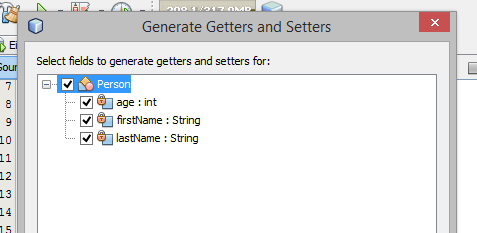
\includegraphics[width=\textwidth]{img/nb005}
\caption{Auswahl der Variablen für die Getter und Setter erzeugt werden sollen}
\label{nb:getset}
\end{figure}
und klicken Sie dann auf "`generate"'. Daraufhin erzeugt die IDE die Getter und Setter. Dies funktioniert in allen IDE's, lediglich der Ort, wo man den Generator findet, ist zuweilen verschieden. 

Mit dem Schreiben solcher Getter und Setter sollte man sich nicht mehr aufhalten. Lassen Sie die IDE dies erledigen. Dann kommen Sie auch nicht in Versuchung, aufgrund von Schreibfaulheit gegen die vorher genannten Regeln zu verstoßen.


\section{Typensystem}\index{Typ}\index{Typisierung}

Java ist eine streng typisierte Sprache (manchmal auch als stark typisiert bezeichnet). Die Definition dieses Begriffs ist leider nicht eindeutig, daher müssen wir ihn hier für uns definieren:

In einer streng typisierten Sprache:
\begin{enumerate}
\item muss jede Variable ei\-nen eindeutigen Typ besitzen,
\item sind Konvertierung von Variablen verschiedener Typen nur in sehr begrenztem, von der Sprache selbst definiertem, Umfang möglich,
\item muss die Typ-Überprüfung zum Zeitpunkt des Kompilierens durchgeführt werden.
\end{enumerate}

Diese Definition mag für manchen entweder nicht ausreichend, oder zu streng sein. Darüber kann man diskutieren. Für die Zwecke in diesem Buch möchte ich die Typisierung in dieser Form definieren, denn sie wird zum einen erklären, warum wir nicht deklarierte Variablen nicht verwenden dürfen. Und zum anderen, warum wir beliebige Objekte nicht in andere Objekte umwandeln können.

\subsection{Konvertierung}\label{ref:conversion}\index{Konvertierung}
TODO


\subsection{Autoboxing und Unboxing}\label{ref:autoboxing}\index{Autoboxing}\index{Unboxing}
TODO


\section{Generics}\index{Generics}
TODO

\section{Unser Projekt}

Für das in der Einleitung beschriebene Projekt brauchen wir (unter vielen anderen Dingen) eine Möglichkeit, mit komplexen Zahlen zu rechnen. Wir könnten natürlich immer mit zwei reellen Zahlen arbeiten, bzw. ihren endlichen Entsprechungen in einem Computer: "`float"' oder "`double"'. 

Aber wir möchten das etwas eleganter gestalten. Wir möchten eine Complex Klasse in der selben Art, wie es eine Double Klasse gibt. Der Anfang hierzu ist relativ einfach: 
\begin{lstlisting}
public class Complex {
  private double real;
  private double imaginary;
}
\end{lstlisting}
Erzeugen Sie hierzu nur die Getter und nicht die Setter. Wählen Sie dafür wie in Abschnitt \ref{chap:getset} die "`Insert Code ..."' Funktion und wählen Sie nicht "`Getter and Setter"', sondern nur "`Getter"'. Das führt dazu, dass eine einmal erzeugte Complexe Zahl nicht mehr verändert werden kann. Ganz so, wie es unserer Vorstellung entspricht, denn Zahlen sollten ihren Wert nicht ändern. Man kann mit ihnen Operationen ausführen, sodass neue Zahlen damit errechnet werden können. Aber dies ändert nicht den Wert der an der Operation beteiligten Zahlen. 

Um es ganz sauber zu machen, müssten wir die Variablen real und imaginary als \texttt{final} deklarieren, dies würde dazu führen, dass selbst wenn wir versuchten die Werte zu verändern, es nicht könnten. Denn ein einmal zu einer als "`final"' deklarierten Variable zugewiesener Wert kann nicht mehr verändert werden.

Um zu verhindern, dass nun irgendein Wert zugewiesen wird, auf den wir keinen Einfluss haben, ist es notwendig, die Variablen im Konstruktor mit Werten zu belegen. Haben wir real und imaginary als "`final"' deklariert, wird uns dies auch der Kompiler schon mitteilen. 
\begin{lstlisting}
public class Complex {
  private final double real;
  private final double imaginary;
  
  public Complex(double re, double im) {
    real = re;
    imaginary = im;
  }
}
\end{lstlisting}
So wird aus unserer Complex Klasse eine Unveränderliche. In späteren Kapiteln werden wir feststellen, dass viele Klassen auf diese Weise unveränderlich sind. Zum Beispiel Zeichenketten (String).

Wie schreiben wir nun Funktionen für die grundlegenden Rechenarten? Die naive Form wäre dies so zu tun:
\begin{lstlisting}
  public Complex add(Complex a, Complex b) {
    return new Complex(a.getReal()+b.getReal(), 
      a.getImaginary()+b.getImaginary());
  }
\end{lstlisting}
Hier haben wir nur die Regel aus Formel (\ref{eq:cmlxadd}) angewendet. Aber diese Funktion ist in keiner Weise vom Status ihrer Instanz abhängig. Daher würde die Anwendung so geschehen müssen:
\begin{lstlisting}
a.add(a,b);
\end{lstlisting}
oder
\begin{lstlisting}
b.add(a,b);
\end{lstlisting}
also was denn nun? Wie wir sehen haben wir da etwas seltsames. Denn die Funktion add() ist unabhängig von ihrer zugehörigen Instanz. So würde man das auch nicht machen, denn die Addition ist eine Operation, die wir mit einer Zahl im Kontext einer anderen ausführen. Der Begriff "`Kontext"' sollte einen sofort wachsam werden lassen, denn der Kontext eines Objekts ist immer der Status seiner internen Variablen. Die naheliegende Implementierung sollte also auf den internen Status des Objekts zugreifen:
\begin{lstlisting}
  public Complex add(Complex b) {
    return new Complex(real+b.getReal(), imaginary+b.getImaginary());
  }
\end{lstlisting}
Und somit ist der Aufruf eindeutig, wir berechnen a+b
\begin{lstlisting}
a.add(b);
\end{lstlisting}
Aufgrund dessen, dass a und b den identischen Typ haben, könnten wir auch 
\begin{lstlisting}
b.add(a);
\end{lstlisting}
berechnen und bekämen dasselbe heraus. Das liegt aber an der Kommutativität der Addition, für die Division stimmt das schon nicht mehr.

In der gleichen Art brauchen wir auch noch die Multiplikation, wie in Formel (\ref{eq:mand}) dargestellt, müssen wir eine komplexe Zahl mit sich selbst multiplizieren. Wir könnten eine spezielle Funktion schreiben, die das Quadrat einer komplexen Zahl berechnet. Aber diese könnten wir nur für diese eine Aufgabe verwenden. Wir versuchen immer Funktionen zu schreiben, die die größtmögliche Wiederverwendbarkeit garantieren. Wir realisieren hier die Multiplikation nach Formel (\ref{eq:cmlxmul}). 

\begin{lstlisting}
  public Complex multiply(Complex b) {
    return new Complex(real*b.getReal()-imaginary*b.getImaginary(),
      real*b.getImaginary()+imaginary*b.getReal());
  }
\end{lstlisting}

\section{Aufgaben}
\begin{enumerate}
\item Was ist eine Instanz?
\item Woraus besteht eine Klasse?
\item Welches sind die sogenannten "`primitiven"' Datentypen von Java?
\item Wir haben eine Klasse geschrieben, die einen Konstruktor ohne Parameter besitzt. Wird dann vom Compiler noch ein Default-Konstruktor erzeugt? Warum (nicht)?
\item Welchen Namen hat der Getter für die Variable "`angestellt"' vom Typ "`boolean"'?
\item Welchen Namen hat der Setter für die Variable "`setComplete"' vom Typ "`boolean"'?
\item Welchen Namen hat der Getter für die Variable "`isFinal"' fom Typ "`int"'?
\item Welchen Namen hat der Getter für die Variable "`isFinal"' fom Typ "`boolean"'?
\end{enumerate}






\chapter{Objektorientierte Programmierung}\label{chap:oop}

Ich hatte mich während der Konzeption des Buches zunächst geweigert ein eigenes Kapitel über Objektorientiertheit und/oder objektorientierte Programmierung (OOP) zu schreiben. Ich wollte -- wie in der Einleitung schon beschrieben -- die Konzepte der Programmierung immer anhand des globalen Beispiels erklären, das am Ende der Lektüre dieses Buches heraus kommen soll. 

Für die OOP habe ich mich eines anderen belehren lassen, denn ein Einblick in die Prinzipien der OOP kann vielfach schneller zu einem tieferen Verständnis führen, als dies bei "`inline"' Erklärungen möglich wäre, also Erklärungen, die genau dort auftreten, wo sie benötigt werden. 

\section{Grundprinzipien}

Die OOP besteht aus den folgenden Eigenschaften, vergleiche hierzu den Wikipedia Artikel \cite{wikioop}.

\begin{enumerate}
\item Abstraktion in Form von Klassen
\item Datenkapselung
\item Persistenz
\item Polymorphie 
\item Vererbung
\end{enumerate}

Um diese näher zu verstehen versuchen wir uns anhand eines Beispiels diese Begriffe zu erarbeiten. Betrachten wir ein Studentenwohnheim. Die einzelnen Zimmer dieses Heims wurden nach ein und dem selben Schema gebaut. Es gab also eine Art Schablone dafür, sie sind von der selben "`Klasse"'. Jeder Student bewohnt ein Zimmer dieses Wohnheims und kann es -- im Rahmen der Vorgaben -- für sich selbst einrichten. Das Zimmer selbst ist also seine eigene "`Instanz"' einer abstrakten Zimmerbeschreibung, die durch einen Architekten definiert wurde. 

Dem gegenüber gibt es Gemeinschaftsräume, die von allen benutzt werden. Sie erfüllen eine "`Funktion"', z.B. die Funktion der Säuberung (Waschräume) oder die Funktion der Nahrungsaufnahme (Küche). Diese funktionalen Bereiche gehören zur Klasse des Studentenzimmers, denn ohne Waschraum oder Küche wäre das Zimmer nicht vollständig. 

Der "`Persistenz"' in unserem Beispiel entspricht die Tatsache, dass ein Student in seinem Zimmer sein kann, trotzdem die Küche aktuell nicht benutzt wird. Die Küche kann also nicht als Indikator dafür verwendet werden, um zu entscheiden, ob ein Student sich im Wohnheim aufhält. 

Polymorphie ist ein recht abstraktes Konzept. In der Studentenwohnheim-Metapher gibt es aber funktionale Räume, die polymorph verwendet werden. Zum Beispiel die Toiletten. Jeder Student, unabhängig von seinem oder ihrem Geschlecht, kann sagen "`Ich gehe zur Toilette"'. Männliche und weibliche Studenten meinen dabei aber verschiedene Räume. So hat die Funktion "`Toilette"' zwei Ausprägungen, eine für jedes Geschlecht. Ähnliches gilt für die Küchen, die meist für Stockwerke oder bestimmte Bereiche zur Verfügung stehen. So können zwei verschiedene Studenten, nachdem sie sagten "`Ich gehe in die Küche"', sich in zwei unterschiedlichen Räumen wiederfinden. 

Vererbung hingegen ist wieder ein Konzept zum Zeitpunkt der Planung des Studentenwohnheims. Der Architekt wird vielleicht die Anforderung gehabt haben, verschiedene Arten von Zimmern einzuplanen. So zum Beispiel Zimmer für einzelne Studenten, Zimmer für Pärchen, Zimmer für alleinerziehende Mütter, Zimmer für behinderte Menschen usw. Zunächst wird er die Gemeinsamkeiten der Zimmer definieren: Jedes Zimmer muss eine Tür, ein Fenster und ein Waschbecken haben. Sowie ein Regal, einen Tisch. Aber schon die Betten in jedem Zimmer müssen an die Anforderungen angepasst werden. Sowie ggf. die Tür für Rollstuhlfahrer breiter gemacht werden muss. 

Der Architekt wird also ein prototypisches Zimmer definieren, das als solches nicht gebaut wird, weil es unvollständig ist. Und dann definiert er die eigentlichen Zimmer als Varianten des Prototyps, dabei braucht er sich bei der Definition aber nur um die Unterschiede zum Prototypen zu kümmern. Also das Single-Zimmer ist ein Prototyp-Zimmer erweitert um ein schmales Bett. Das Pärchen-Zimmer ist ein Prototyp-Zimmer mit etwas größerer Grundfläche und einem Zweipersonenbett. Das Zimmer für alleinerziehende Mütter hat ein kleines, separates Zimmer für das Kind, ein Einpersonenbett und eine etwas größere Grundfläche. Und so weiter. 

Das Prototyp-Zimmer ist damit die Basis und die diversen Zimmer die spezialisierten Versionen des Prototyps. Dabei erben die diversen Zimmer die allgemeinen Eigenheiten des Prototyps und fügen Eigenschaften hinzu oder verändern Eigenschaften (dies wird als "`override"' bzw. Überschreiben bezeichnet) des Prototyps. 

\section{Abstraktion}

Nach diesem etwas blumigen Beispiel kommen wir hier zurück auf die Definition der Begriffe: 

Eine Klasse ist die Kombination aus Variablen-Deklaration und Funktionen-Implementierung. Klassen sind Schablonen für ihre Instanzen. Instanzen einer bestimmten Klassen besitzen alle in der Klasse deklarierten Variablen (keine weiteren) und können diesen Werte zuweisen, denn einer Instanz wird Hauptspeicher zugewiesen, in dem die Variablenwerte abgespeichert werden können. Die Implementierung der Funktionen der Klasse teilen sich alle Instanzen.

\section{Datenkapselung}\label{chap:encapsule}

Als Datenkapselung wird die Vorgehensweise begriffen, Daten -- und damit Variablen -- vor direkten Zugriffen zu schützen. Ein "`Verstecken"' von Implementierungsdetails steckt letztlich dahinter. Ob ein Objekt die Werte einer bestimmten Information auch wirklich in einer zugehörigen Variable speichert, oder sich eines grundsätzlich anderen Mechanismus bedient, darf den Benutzer eines Objekts nicht interessieren. Solange der Benutzer einen Getter und Setter für bestimmte Informationen hat und er die Aktionen durchführen kann, wofür er das Objekt verwenden wollte. Dann sollte ihm die Art und Weise egal sein, wie das Objekt letztlich die Durchführung seiner Aktionen  erreicht. Dies ist ein elementarer und sehr zentraler Abstraktionsmechanismus der objektorientierten Programmierung.

Grundvoraussetzung für eine Datenkapselung ist die Kontrolle der Sichtbarkeit von Variablen. Hierfür stehen dem Entwickler von Klassen die Modifikatoren "`public"', "`protected"' und "`private"' zur Verfügung. 

\section{Persistenz}
TODO

\section{Polymorphie}
TODO


\section{Vererbung}\label{chap:inherit}
TODO





\appendix
%    Include appendix "chapters" here.
\include{}

\backmatter
%    Bibliographies can be prepared with BibTeX using amsplain,
%    amsalpha, or (for "historical" overviews) natbib style.
\bibliographystyle{amsalpha}
\bibliography{java-literature}

\printindex

\end{document}

